% !TeX root = ../main.tex
% Add the above to each chapter to make compiling the PDF easier in some editors.

\chapter{Evaluation}\label{chapter:Evaluation}

The goal of this chapter is to validate the framework architecture design for context-aware pervasive computing in challenged environments which was described in Chapter \ref{chapter:Approach}. It also evaluates the middleware implementation which was explained in Chapter \ref{chapter:implementation}. Note that, the delays and performances are to be taken with a grain of salt, as the system is designed as a proof-of-concept and not to run in production systems. \\

\noindent In order to evaluate the framework and implementation with all its requirements, we divided the evaluation into several use cases. The devices used for  the use cases has different hardware capabilities. They might also have  sensors and actuators according to each use case. All the devices must be running our stack framework as explained in \ref{subsec:starting-framework} except for android phones which has \textit{Liberouter}, an implementation for SCAMPI on android phones. The devices we used in this evaluation are:
\begin{center}
	\begin{tabular}{ c | c | c| c }
		
		Name & Count & Stack & Performance \\ \hline
		 &  &  &  \\
		Intel NUC &1& 	Our framework &   \specialcell[c]{CPU:Intel Core i5-6260U Processor\\ (4M Cache, up to 2.90 GHz)\\RAM: 16GB }\\ 
		&  &  &  \\
		Raspberry Pi 3 model B & 2 & Our framework &  \specialcell[c]{ CPU: 1.2GHz\\RAM: 1GB}  \\ 
		&  &  &  \\
		HTC one M9 & 1 & Liberouter &   \specialcell[c]{CPU: Octa-core \\4 x 2.0GHz + 4 x 1.5GHz\\ RAM: 3GB} \\ \hline
	\end{tabular}
\end{center}




\section{Recognizing Water Bottles }
 \begin{figure}[H]
	\centering
	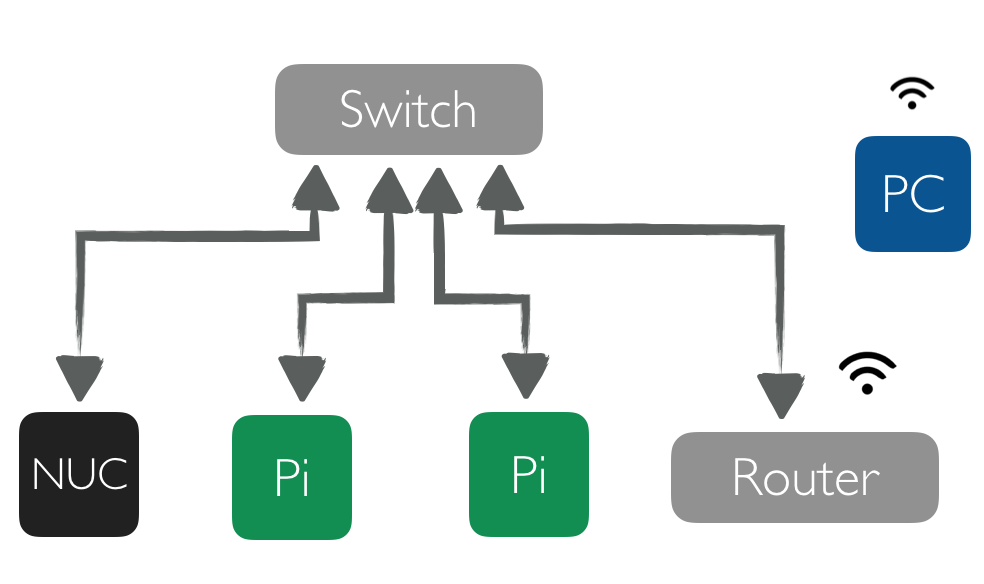
\includegraphics[scale=0.6]{images/tb-tensor.png}
	\caption{Testbed setup for recognizing water bottles.}
	\label{fig:tb-tensor}
\end{figure} 

\section{Challenged Networks}
\begin{figure}[H]
	\centering
	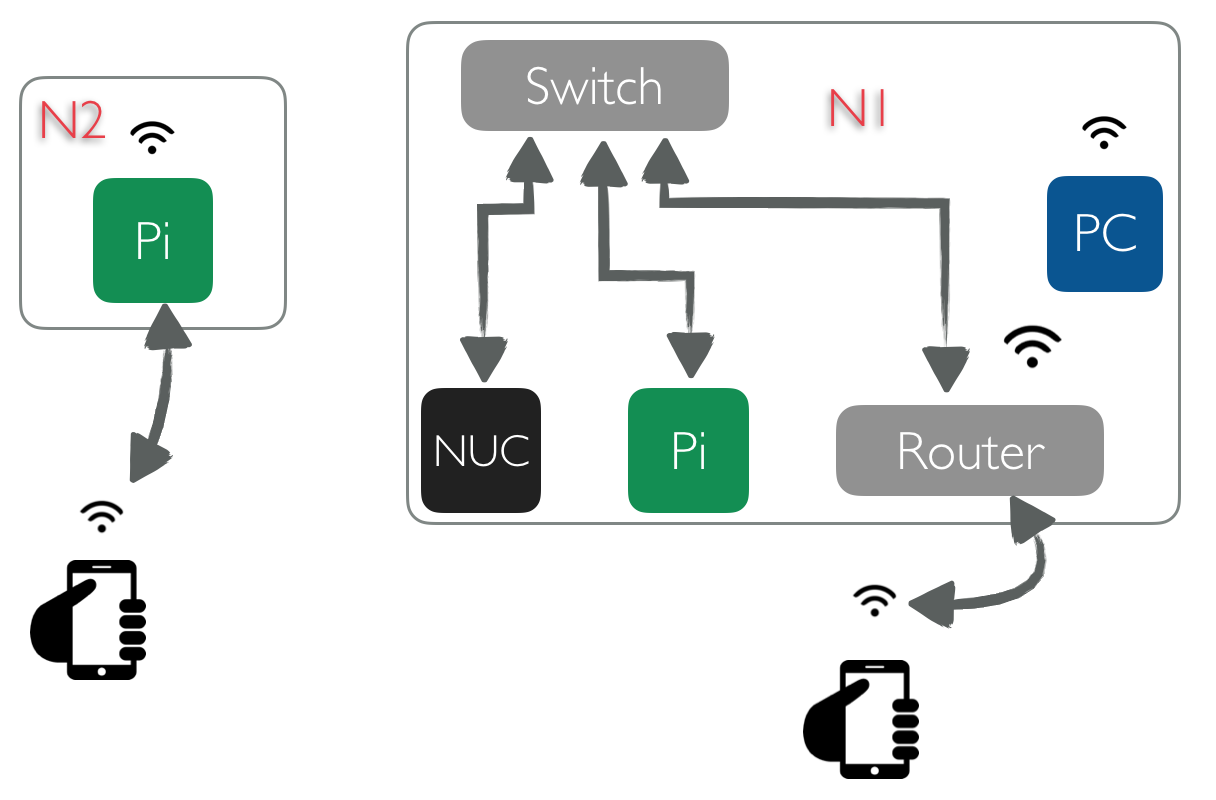
\includegraphics[scale=0.6]{images/tb-dtn.png}
	\caption{Testbed setup for challenged and delay tolerant networks.}
	\label{fig:tb-dtn}
\end{figure} 

\section{Basic IoT Usage}